\documentclass[parskip=full]{scrartcl}

\usepackage[utf8]{inputenc} % use utf8 file encoding for TeX sources
\usepackage[T1]{fontenc} % avoid garbled Unicode text in pdf
\usepackage[german]{babel} % german hyphenation, quotes, etc
\usepackage{hyperref} % detailed hyperlink/pdf configuration
\hypersetup{ % ‘texdoc hyperref‘ for options
pdftitle={Lamb.da - Das Spiel}
}
\usepackage{csquotes} % provides \enquote{} macro for "quotes"
\usepackage{graphicx}

\usepackage{enumerate}

\begin{document}

\title{Lamb.da - Das Spiel}
%\date{October 12, 123}
\author{Name, Name, Name}
\maketitle

\section{Einleitung}

\section{Zielbestimmung}

\subsection{Musskriterien}

\subsection{Wunschkriterien}

\subsection{Abgrenzungskriterien}
\section{Produkteinsatz}

\subsection{Anwendungsbereiche}

\subsection{Zielgruppen}

\subsection{Betriebsbedingungen}
\section{Produktumgebung}

\subsection{Software}
\begin{itemize}
	%4.2 evtl. ersetzen 
	\item Das Produkt wird für Android entwickelt und sollte auf allen Versionen ab 4.2 (4.2 oder höher) laufen.
\end{itemize}

\subsection{Hardware}
\begin{itemize}
	\item Das Programm ist für Smartphones und Tablets konzipiert
	%sonst noch irgendwas? Hardware-Anforderungen?
\end{itemize}

\section{Funktionale Anforderungen}
% TODO FA Nummern anpassen

\subsection{Profile}

Profile ermöglichen das Nutzen des Programms durch mehrere Anwender auf demselben Gerät.

\begin{itemize}
\item /FA110/ Jeder Nutzer soll ein eigenes Profil angelegen können, welches eindeutig durch den Profil-Namen gekennzeichnet ist. 
\item /FA120/ Bei Programmstart wird das zu benutzende Profil ausgewählt oder ein neues Profil erstellt.
\item /FA130/ Die zu einem Profil gespeicherten Daten können nach Erstellen des Profils geändert werden.
\item /FA140/ Ein Profil kann nach dem Erstellen wieder gelöscht werden.
\item /FA150/ Zu jedem Profil werden Spieleinstellungen, Spielfortschritt und Spielstatistik gespeichert.
\item /FA150/ Beim Auswählen eines Profils werden die dazu gespeicherten Daten automatisch geladen.
\item /FA160/ Nach dem Auswählen eines Profils wird der Nutzer durch eine profilspezifische Nachricht begrüßt.
\end{itemize}

\subsection{Spielmodi}

Im Editor-Modus werden Terme erstellt, angezeigt und bearbeitet.

\begin{itemize}
\item /FA211/ Durch Ziehen können Objekte sowohl von der Werkzeugleiste als auch vom Term ausgewählt werden.
\item /FA212/ Während ein Objekt ausgewählt ist, wird die aktuelle Stelle im Term, an der das Objekt platziert werden kann, farblich markiert.
\item /FA213/ Während ein Objekt ausgewählt ist, kann durch Loslassen des Zeigers das Objekt an der aktuellen Stelle im Term platziert werden.
\item /FA214/ Während ein Objekt ausgewählt ist, kann durch Loslassen des Zeigers über der Werkzeugleiste das Objekt gelöscht werden.
\item /FA215/ Neu hinzugefügte Objekte erhalten die Farbe weiß.
\item /FA216/ Durch Drücken eines Objektes wird ein Popup-Fenster geöffnet, in dem eine neue Farbe für das Objekt ausgewählt werden kann.
\item /FA217/ Das Ändern der Position oder Farbe von durch ein Level vorgegebenen Objekten kann optional unterdrückt werden.
\item /FA217/ Gültige Terme enthalten keine weißen Objekte.
\end{itemize}

Im Reduktions-Modus werden Terme schrittweise durch Beta-Konversionen reduziert.

\begin{itemize}
\item /FA221/ Durch Drücken des Vorwärts-Knopfes wird eine einzelne Konversion ausgeführt.
\item /FA222/ Durch Drücken des Rückwärts-Knopfes wird der Term auf den Zustand vor der zuletzt ausgeführten Konversion zurückgesetzt.
\item /FA223/ Durch Drücken des Abspielen-Knopfes werden automatisch nacheinander schrittweise Konversionen duchgeführt bis keine Reduktionen mehr möglich sind oder der Pause-Knopf gedrückt wurde.
\end{itemize}

\subsection{Level}

Das Spiel ist in Level eingeteilt, welche vom Spieler nacheinander freigeschaltet und gelöst werden.

\begin{itemize}
\item /FA231/ Das Ziel des Leveltyps "`Eingabe-Bestimmung"' ist es, im Editor-Modus einen gültigen Term zu erstellen, welcher durch Konversionen im Reduktions-Modus in einen minimalen im Level vorgegebenen Term umgewandelt wird.
\item /FA232/ Das Ziel des Leveltyps "`Ausgabe-Bestimmung"' ist es, im Editor-Modus einen gültigen Term zu erstellen, welcher aus der Reduktion eines im Level vorgegebenen Terms hervorgeht.
\item /FA233/ Nur das erste Level ist nach Erstellung eines Profils freigeschaltet, durch Abschließen eines Levels wird das darauf folgende Level freigeschaltet.
\item /FA234/ Nach erstmaligem erfolgreichen Abschließen eines Levels wird automatisch das darauf folgende Level gestartet.
\item /FA235/ Nach erfolgreichen Abschließen eines Levels wird der Spieler durch ein Popup-Fesnter über den Erfolg informiert.
\item /FA235/ Nach erstmaligem erfolgreichen Abschließen des letzten Levels wird dem Spieler durch ein Popup zu seiner Leistung gratuliert.
\item /FA236/ Über ein Level-Menu kann der Spieler seinen Level-Fortschritt beobachten und bereits freigeschaltete Level erneut spielen.
\item /FA237/ Die Level sind in verschiedene Schwierigkeitsstufen eingeteilt, welche durch Farbe und Hintergrundbild voneinander unterscheidbar sind.
\item /FA238/ Über einen Hinweis-Knopf kann sich der Spieler Tipps und Lösungsansätze zu dem aktuellen Level anzeigen lassen.
\end{itemize}

\subsection{Gamification}

Durch ein Belohnungssystem wird die Spiel- und Lernfreude der Nutzer verbessert.

\begin{itemize}
\item /FA241/ Das erstmalige Abschließen eines Levels wird mit einer Level-spezifischen Anzahl von Münzen belohnt.
\item /FA242/ Im Shop kann kann der Nutzer gegen Eintausch von Münzen neue Sounds, Hintergrundbilder und Avatare freischalten.
\item /FA242/ Vor dem freischalten eines Elements im Shop wird der Spieler um eine Bestätigung gebeten.
\item /FA243/ Im Shop freigeschaltete Elemente können dort durch ein Kontrollkästchen aktiviert werden. Standardmäßig werden gerade gekaufte Sounds oder Hintergrundbilder sofort aktiviert.
\item /FA244/ Für bestimmte Leistungen werden Erfolgsnachrichten in einem Achievement-Menu angezeigt. Folgende Erfolge sind möglich:
\begin{itemize}
\item Alle Level eines Schwierigkeitsgrades abgeschlossen.
% TODO
\end{itemize}
\item /FA244/ Im Ladebildschirm werden zur Unterhaltung des Nutzers Comic-artige Sprechblasen mit lustigen und interessanten Texten angezeigt.
\end{itemize}

\subsection{Eltern und Lehrer}

Statistiken und Optionen für Eltern und Lehrer geben diesen einen Einblick in den Lernfortschritt des Kindes.

\begin{itemize}
\item /FA231/ In einem Statistik-Menu werden verschiedene Daten angezeigt. Folgende Daten sind möglich:
\begin{itemize}
\item Spielzeit
\item Anzahl Versuche gesamt
\item Erfolgsquote für das Bestehen der Level
\item Häufigkeit der Nutzung von Hinweisen
% TODO
\end{itemize}
\item /FA231/ Über den Lehrermodus wird im Editor sowie im Reduktions-Modus der aktuelle Lambda-Term in mathematischer Darstellung angezeigt.
\end{itemize}

\subsection{Benutzerinteraktion}

\begin{itemize}
\item /FA231/ Über den Touchscreen des Gerätess kann der Nutzer mit dem Programm interagieren.
\item /FA238/ Über den Lautstärkeregler des Gerätes kann die Lautstärke des Programms verändert werden.
\item /FA238/ Mit dem "`Zurück-Knopf"' des Gerätes kann in der Menu-Auswahl in das vorherige Menu gewechselt werden.
\item /FA238/ Mit der Drag\&Drop-Geste kann im Editor der Term auf dem Bildschirm verschoben werden.
\item /FA238/ Mit die Pinch-Geste kann im Editor die Zoomstufe verändert werden.
\item /FA238/ Über einen Knopf im Hauptmenü kann die Hintergrundmusik an- und ausgeschaltet werden.
\item /FA238/ Das Programm unterstützt das Auswählen der Sprachen Englisch, Deutsch und Französisch.
\end{itemize}
\section{Produktdaten}
% TODO L und LD Nummern anpassen

Alle Daten werden Profil-spezifisch gespeichert.

\begin{itemize}

\item /D10/ Profil
\begin{itemize}
\item /LD10/ Profilname
\item /LD10/ Avatar
\item /LD10/ Sprache
\end{itemize}

\item /D10/ Spieloptionen
\begin{itemize}
\item /LD10/ Lehrermodus aktiviert
\item /LD10/ Hintergrundmusik aktiviert
\end{itemize}

\item /D10/ Spielfortschritt
\begin{itemize}
\item /LD10/ Letztes freigeschaltetes Level
\item /LD10/ Abgeschlossene Achievements
\end{itemize}

\item /D10/ Statistik
\begin{itemize}
\item /LD10/ Gesamtanzahl der Versuche
\item /LD10/ Erfolgreiche Versuche
\item /LD10/ Zeit im Editor verbracht
\item /LD10/ Zeit im Reduktions-Modus verbracht
\item /LD10/ Gesamtzeit im Programm verbracht
\item /LD10/ Anzahl von genutzten Hinweisen
% TODO
\end{itemize}

\end{itemize}
\section{Nichtfunktionale Anforderungen}

\begin{itemize}
\item \textbackslash NF10 \textbackslash Anforderungsbeschreibung
\end{itemize}
\section{Systemmodelle}

\subsection{Globale Testfälle}
Folgende Funktionssequenzen sind zu überprüfen:

\begin{itemize}
\item \textbackslash T10 \textbackslash Funktionssequenzbeschreibung
\end{itemize}

\subsection{Datenkonsistenzen}

\begin{itemize}
\item \textbackslash T30 \textbackslash Datenkonsistenzbeschreibung
\end{itemize}

\subsection{Objektmodell}
% UML Klassendiagramme

\begin{figure}[h]
\centering
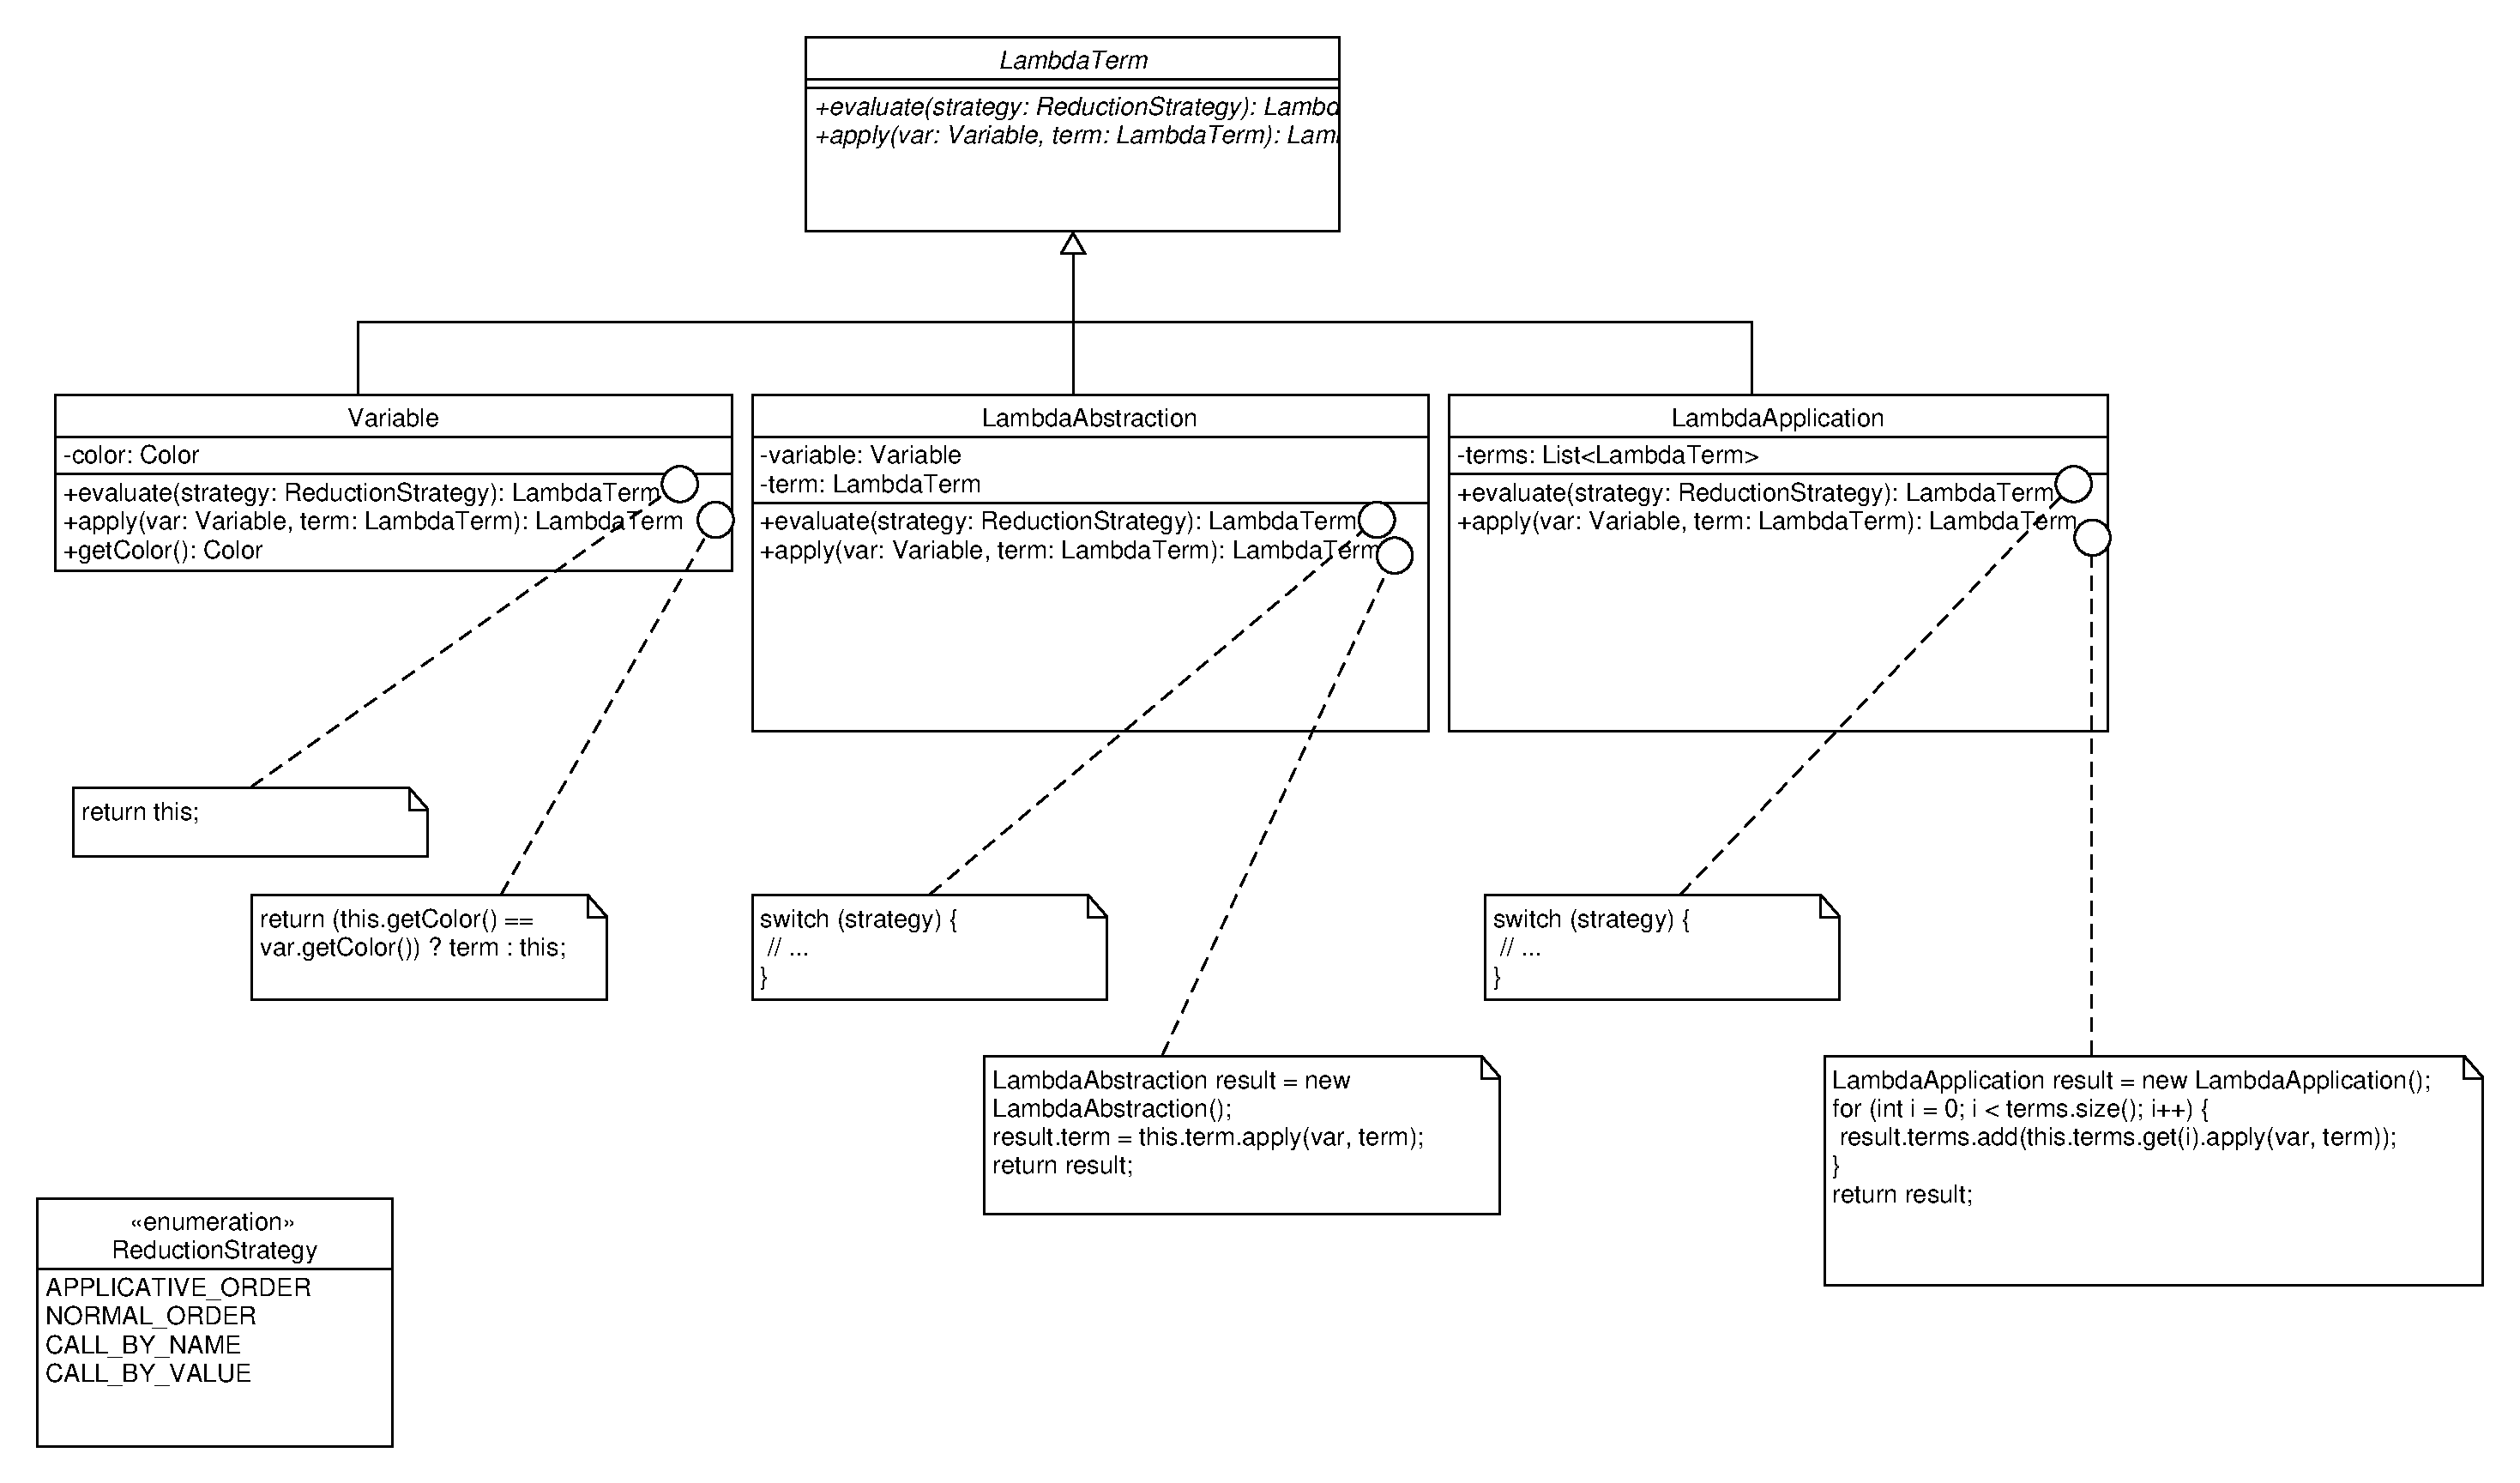
\includegraphics[scale=0.35]{../system_models/object_models/lambda_calculus.pdf}
\caption{UML Klassendiagramm zum Lambda-Kalkül}
\end{figure}

\subsection{Dynamische Modelle}
% UML Zustandsautomat, Sequenzdiagramm

\begin{figure}[h]
\centering
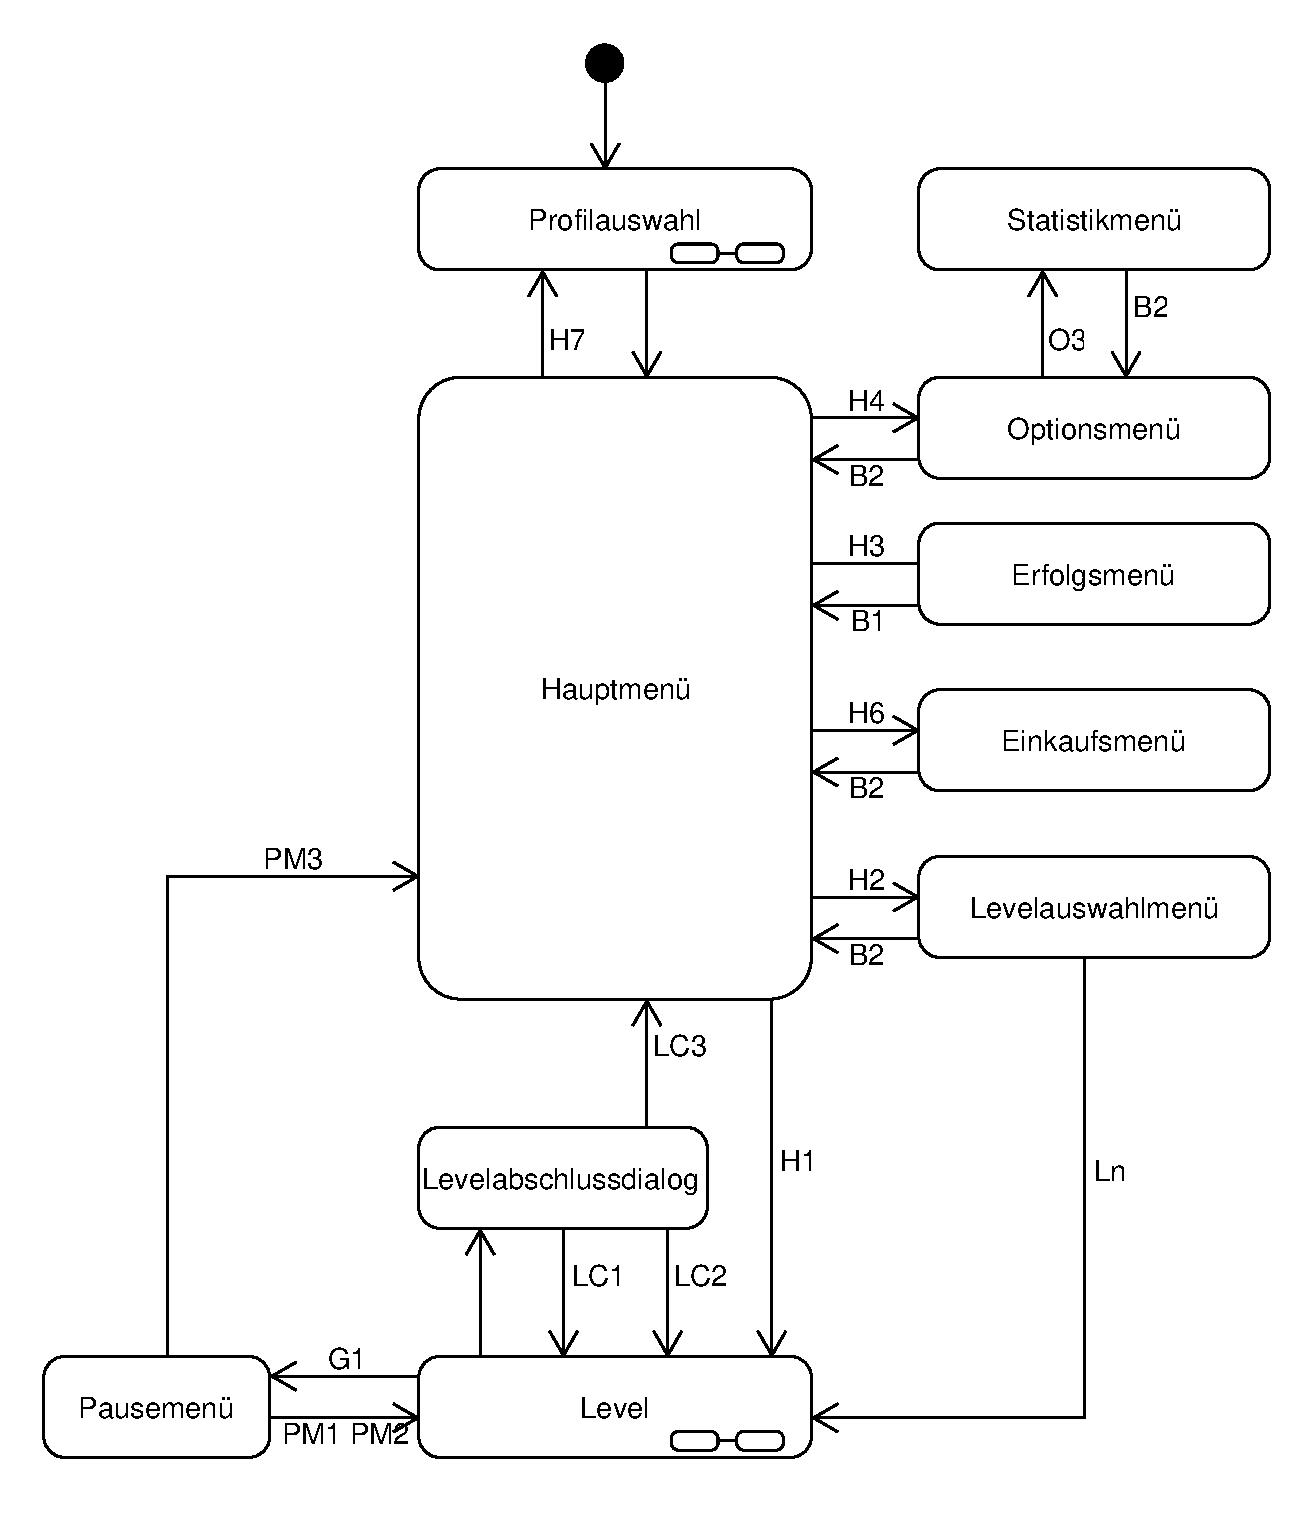
\includegraphics[scale=0.3]{../system_models/dynamic_models/menu_state_machine.pdf}
\caption{Zustandsautomat zur Menübedienung}
\end{figure}

\begin{figure}[h]
\centering
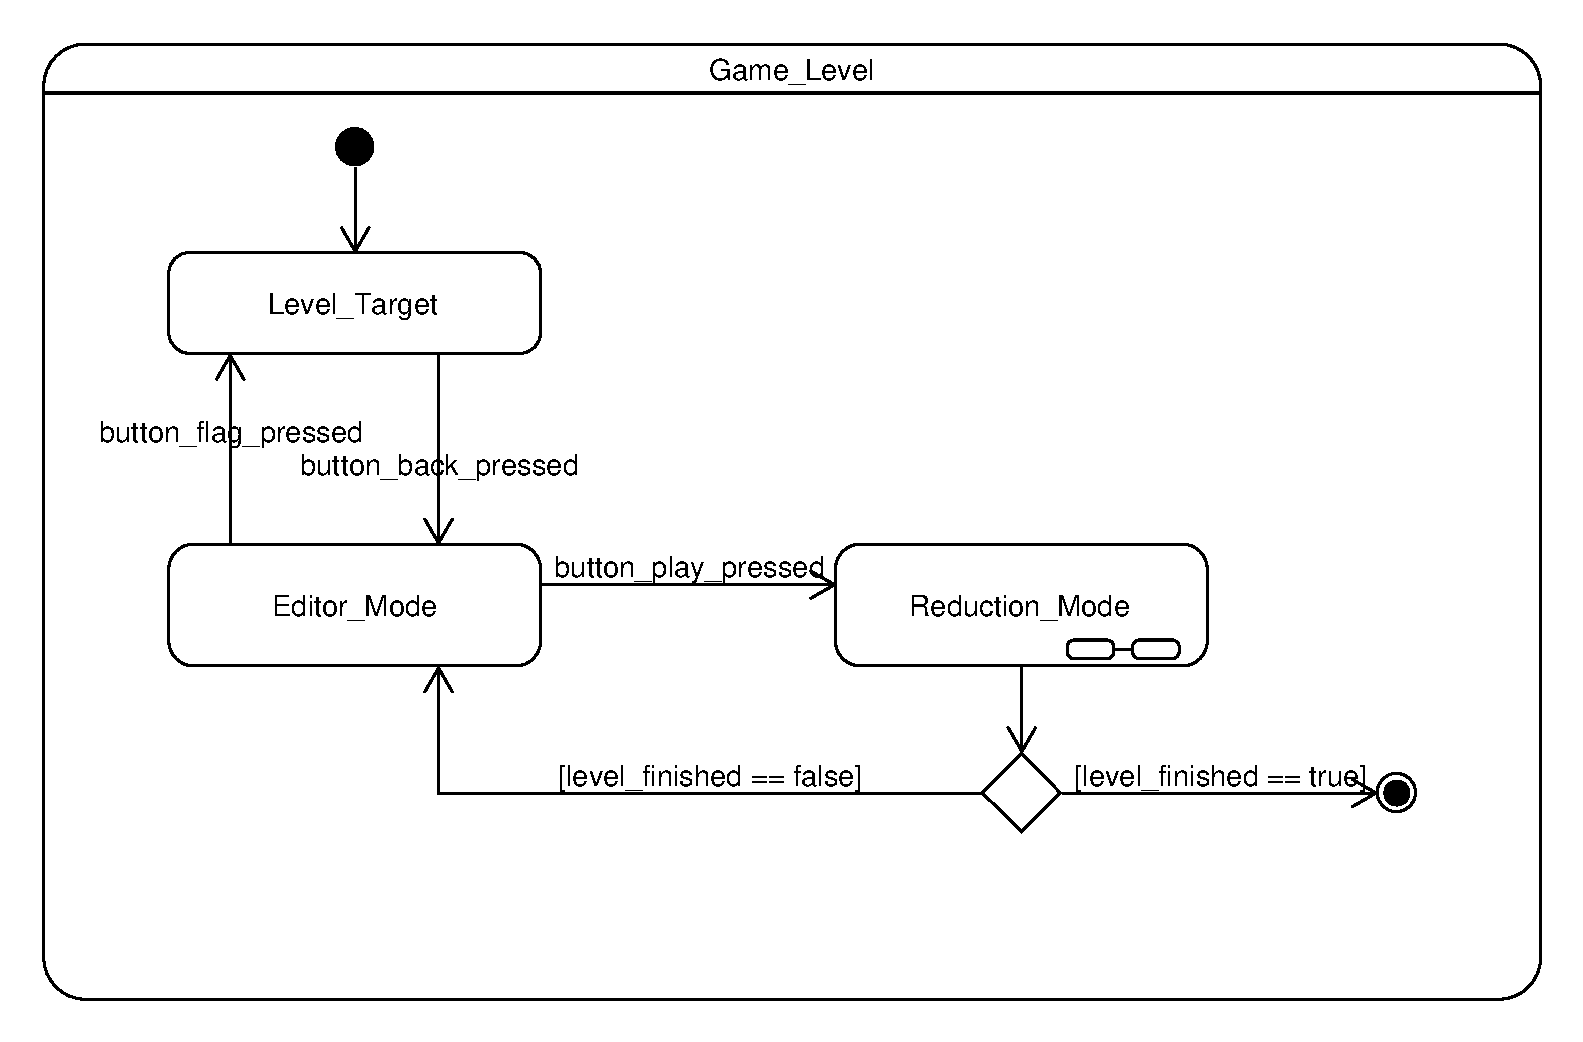
\includegraphics[scale=0.6]{../system_models/dynamic_models/game_level_state_machine.pdf}
\caption{Zustandsautomat zum Ablauf eines Levels}
\end{figure}

\begin{figure}[h]
\centering
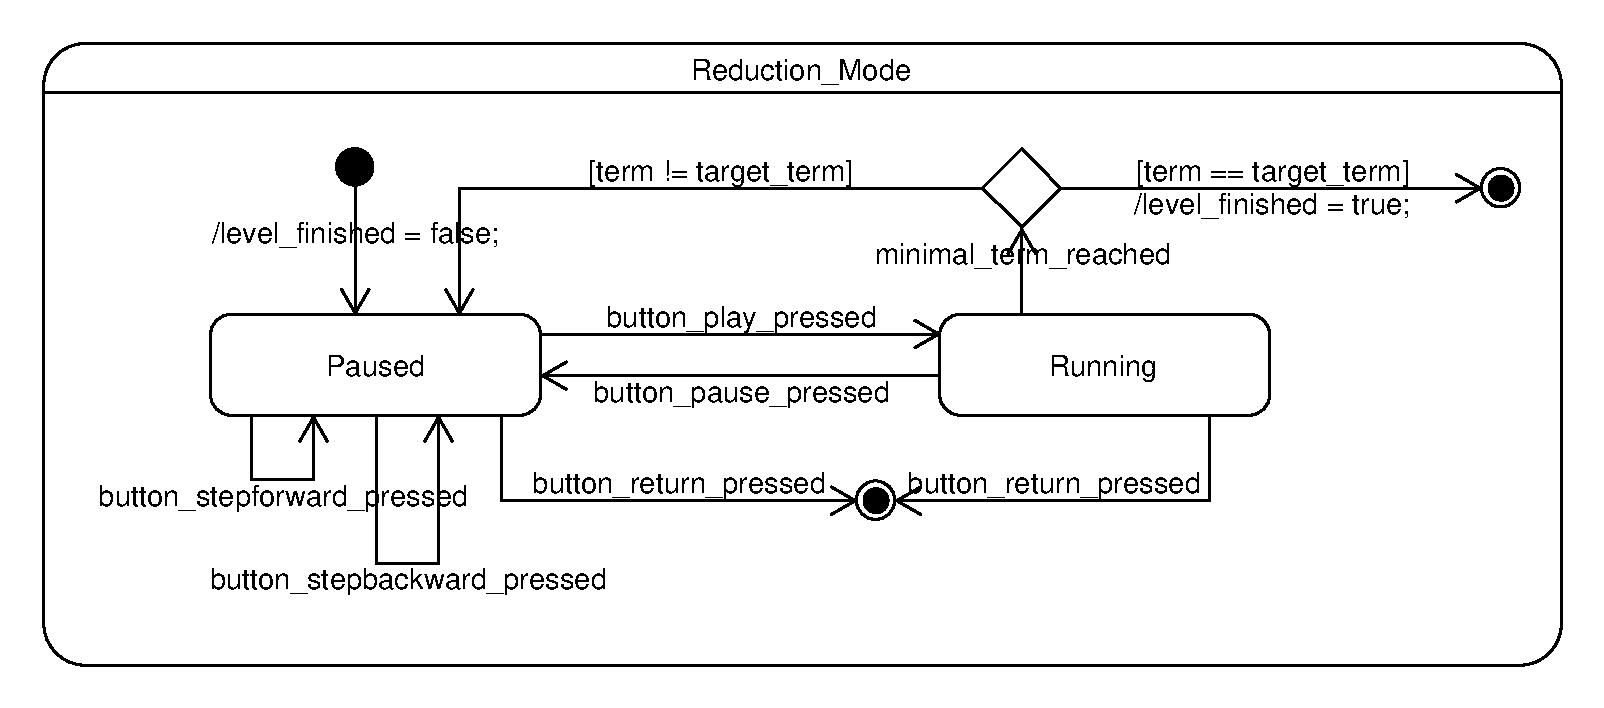
\includegraphics[scale=0.6]{../system_models/dynamic_models/reduction_mode_state_machine.pdf}
\caption{Zustandsautomat zur Funktion des Reduktions-Modus}
\end{figure}

\subsection{Benutzerschnittstelle}

GUI
\section{Glossar}


\end{document}